\label{sec:empirical}
% Empirical	Approach
% Description of the empirical model: specification and variables involved
% Strategy for the estimation of the parameters of interest and test of the hypothesis
\subsection{Network Characteristics}
We start by characterizing the network. Recall, that we view airports as nodes, and flights between airports as edges. Considering the dataset of flights in 2007 from the 2009 Statistical Computing Data Expo, we produce a network of US airports and the flights connecting them. We will refer to this network as the US Network. This network has 310 nodes and 2868 edges. With 310 nodes, the maximum possible number of edges would be (\cite{Barabasi Networks}): 
\begin{align}
    L_{max}  = \frac{N\cdot(N-1)}{2}=\frac{310\cdot(310-1)}{2} = 47.895
\end{align}
This implies, that only approximately 5,9 pct. of possible edges are actually found in the network. 
% Tjek nedenstående når vi ved mere
This sparseness of the network seems to support the hub-and-spoke nature of air transport; rather than having all airports be connected, it is more economically sensible to have certain airports function as hubs in their geographical area, and connect to hubs in other regional areas. \\ 
To get a further sense of how the network is connected we calculate the degree centrality for each node in the network, that is the number of other airports each airport is connected to through flights in 2007. \\
The average degree for the 310 airports contained in the dataset is 18,5. This average masks a huge variation; the highest degree found in the dataset is the Hartsfield-Jackson Atlanta International Airport (ATL) with a degree of 186. This airport is also listed as the busiest airport in the world by landings and take-offs by Airports Council International \footnote{https://aci.aero/data-centre/monthly-traffic-data/aircraft-movements/year-2017/12-months/}. Conversely, 51 airports have a degree of 1, implying that in this dataset they only appear in connection with a single other airport. \\
The degree distribution can be seen in the figure below. Clearly, a large number of airports are connected by flights to few other airports, while a minority of airports are much more connected. \\

As an alternative measures of centrality in the network, we calculate \textit{betweenness centrality} that measures the degree to which an edge is part of the shortest path between two other edges where path length is defined as the number of traversed links. \\
In the end, we use clustering coefficient, betweenness and degree as features in the prediction model. Note, that these are all node-specific measures, and as such, for each observation, there are two of each corresponding to origin and destination airport. 

% Figur med hhv. degree distribution (til venstre) og betweenness centrality (højre)?

\subsection{Network vulnerability}
We conduct an analysis of how the network is affected when certain nodes are removed. This analysis is, broadly, in line with the analysis in \cite{chi2004structural}. \\
The figure below shows how key network characteristics (average degree, clustering coefficient and global efficiency) are affected, when nodes are removed. One curve corresponds to removal of the most connected nodes, this is what we refer to as an 'attack' on the network, where the hubs are targeted. \\
Secondly, we consider how the network is affected when we remove the least important nodes first. \\
Finally, we consider how the network is affected by an event that removes all network in a geographical area (such as might be the case due to natural disaster og extreme weather conditions). We conduct this analysis by choosing a spot in the continental US, calculating the (geographical) distances from each airport to this spot, and then removing all airports within x miles. This final analysis takes advantage of the spatial nature of the network, and provides insight into how geographically determined failures may affect the network. \\
It should be noted, that in this section we analyze the network as it is in our dataset. Obviously, were a number of airports to close for a prolonged period (e.g. due to natural disaster), the agents in the market would make changes to the network to accommodate the new situation. Market forces is likely to have been a determinant in producing the network as is, and exogenous changes to the network would cause changes in behaviour of the agents in the market, that would produce a new network. \\ 

\begin{figure}[H]
  \centering
  \caption{Fully-connected point-to-point network vs hub-and-spoke network}
    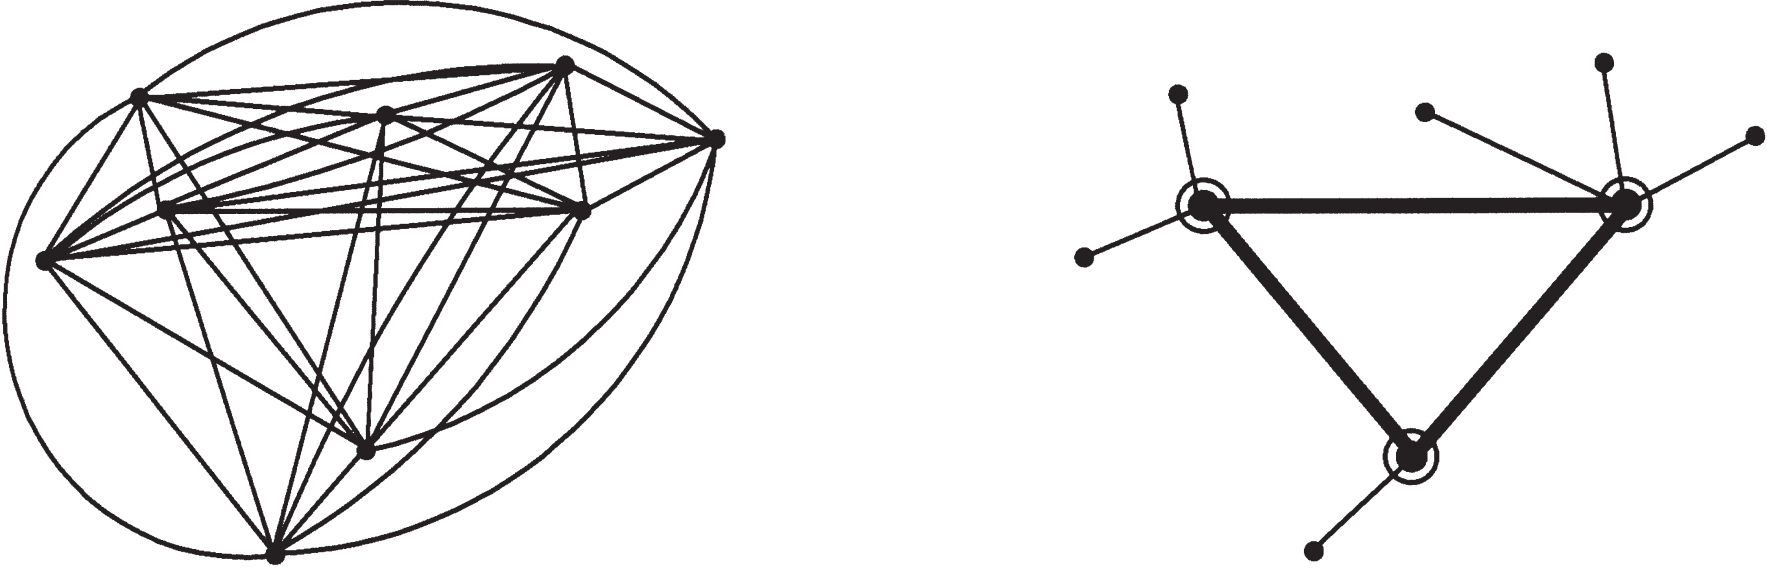
\includegraphics[width=1. \textwidth]{03_figures/Bryan_1999_networks}
    \sourcecenter{\citet{bryan1999hub}}
  \label{fig:different_networks}
\end{figure}

\subsection{Predicting Flight Prices - Do Network-related Features add Predictive Power?}
Our set of network-related features includes, for both origin and destination airport: Betweenness centrality, degree and clustering coefficient. \\
Our set of other features includes: The number of flights on the given route in the year considered, the distance between the two airports, the (average) time in minutes for the flight and the number of carriers who flew the route during the year considered. \\
Our key question is then whether or not adding the network-related features contributes predictive power in predicting prices. 
